\documentclass[headinclude,DIV12]{scrartcl}

\usepackage[latin1]{inputenc}
\usepackage[T1]{fontenc}
\usepackage[english]{babel}
\usepackage{textcomp}

\usepackage{scrpage2}
\usepackage{url}
%
\usepackage{pst-optexp}
\let\verPstOptExp\fileversion
\let\datePstOptExp\filedate
\usepackage{multicol}
\usepackage{showexpl}
\lstset{breakatwhitespace}
\usepackage{nicefrac}
\usepackage{graphicx}
\usepackage{array}
\usepackage{longtable}
\usepackage{booktabs}
\usepackage[colorlinks,linktocpage]{hyperref}
%
% New commands
%
\DeclareRobustCommand\cs[1]{\texttt{\char`\\#1}}
\newcommand{\OptExpPackage}{\textsf{`pst-optexp'}}
\newcommand{\parameter}[1]{\texttt{#1}}
\let\param\textrm
\newcommand{\paramvalue}[1]{\texttt{#1}}
\newcommand{\defaultparam}[1]{\emph{default:} \paramvalue{#1}}
\def\lbracket{[}
\def\rbracket{]}
\newcolumntype{T}{>{\ttfamily}l}
\newcolumntype{B}{>{\bfseries}l}
%
% Settings
\setkomafont{sectioning}{\normalfont\normalcolor\bfseries}
%
\makeatletter
\renewenvironment{description}
  {\list{}{\labelwidth\z@ \itemindent-\leftmargin
    \itemsep0pt \parsep0pt
    \let\makelabel\descriptionlabel}}
  {\endlist}
\makeatother
%
\clearscrheadfoot
\setheadsepline{0.4pt}
\ihead{\OptExpPackage}\ohead{A PSTricks package to draw optical experimental setups}
\ofoot{\pagemark}
\pagestyle{scrheadings}

\psset{subgriddiv=0,griddots=10,gridlabels=7pt}

%%%%%%%%%%%%%%%%%%%%%%%%%%%%%%%%%%%%%%%%%%%%%%%%%%%%%%%%%%%%%%%%%%%%%%%%
\begin{document}
 \title{\texttt{pst-optexp}\\ A PSTricks package to draw optical experimental setups}
 \author{Christoph Bersch \textless
   \href{mailto:usenet@bersch.net}{\texttt{usenet@bersch.net}}\textgreater}
 \date{\datePstOptExp\enspace\enspace Version \verPstOptExp}

\maketitle

\setlength{\columnseprule}{0.6pt}
\begin{multicols}{2}
{\parskip 0pt \tableofcontents}
\end{multicols}
\section{Introduction}
The package \texttt{pst-optexp} is a collection of optical components
that facilitate easy sketching of optical experimental
setups. Mechanisms for proper alignment of different components are
provided internally. This way the user does not have to care for proper
orientation of the elements. Macros for convenient definition of new 
user-defined components are also provided.

\section{Concept and General Options}\label{sec:general}

\subsection{Concept}

There are two different categories of optical components that are
provided by the package: free-ray and fiber-optical components.  

The free-ray components are subdivided in two different kinds: the
components which require two reference points and do not alter the
direction of the passing light beam (e.g. lenses and retardation plates)
and those which work in reflection and require three reference points
(mirrors, gratings, beamsplitters etc.). 

For free-ray setups one usually has few straight light paths in which
several different components are arranged. Therefore, it is more
convenient if one has to define only two nodes for each light path. The
components then are placed on this light path using the different
positioning parameters of the package and at the end the beam itself is
drawn. This concept is different from the one used for the fiber-optical
components or the way \texttt{pst-circ} treats its objects. They
directly connect the components with the reference nodes.

The fiber-optical components can be subdivided in dipoles, tripoles and
quadrupoles which have a corresponding number of fiber connections. The
handling of these components differs in some aspects from the free-ray
objects. The fiber optics are directly connected with the reference
nodes. The psstyles used for each fiber connections can be flexibly
changed for every components (see sec. \ref{sec:styles}).

Some hybrid components (laser, optbox, detector etc.) can be used both
as fiber-optical or free-ray elements. By default they are treated as
free-ray objects, i.e. they are not connected to their reference
points. Setting the parameter \parameter{fiber} to \parameter{true} they
are treated as fiber-optical object and connected with the reference
points using the appropriate psstyles.

\subsection{General Options}
\begin{description}
\item[\param{angle}:] \paramvalue{<value>} (\defaultparam{0})
\item[\param{optional}:] \paramvalue{<boolean>} (\defaultparam{false})
\item[\param{position}:] \paramvalue{<value>} (\defaultparam{\cs{@empty}})
\item[\param{abspos}:] \paramvalue{<value>} (\defaultparam{\cs{@empty}})
\item[\param{showoptdots}:] \paramvalue{<boolean>} (\defaultparam{false})
\item[\param{fiber}:] \paramvalue{<boolean>}
\item[\param{extnode}:] \paramvalue{<ref string>} (\defaultparam{\cs{@empty}})
\item[\param{extnodename}:] \paramvalue{<string>} (\defaultparam{Ext})
\end{description}

The parameter \parameter{angle} is available for the macros \cs{optbox}
and \cs{crystal} only, as for the most other cases it would make
no sense. \parameter{optional} can be used with every component and marks it as
optional and can be configured by changing the psstyle \parameter{OptionalStyle}.
\parameter{position} is equivalent to the \parameter{npos} parameter of \cs{ncput},
but is used only for the \lq dipole\rq-macros to position the component
between the two given points. In addition, there is a parameter
\parameter{abspos} that allows absolute positioning between the two line
points. \parameter{showoptdots} shows in black the two points calculated for the
positioning of the component, and in red the reference points for the
label.

\medskip

\begin{LTXexample}[width=3.5cm]
\begin{pspicture}(3,2)\psgrid
  \pnode(0,1.2){A}
  \pnode(3,1.2){B}
  \psline[style=Beam](A)(B)
  \optbox[angle=10](A)(B){box}
\end{pspicture}
\end{LTXexample}

\bigskip

\begin{LTXexample}[width=3.5cm]
\begin{pspicture}(3,2)\psgrid 
  \pnode(0,1.2){A} 
  \pnode(3,1.2){B}
  \psline[style=Beam](A)(B) 
  \lens[optional](A)(B){L}
\end{pspicture}
\end{LTXexample}

\bigskip

\begin{LTXexample}[width=3.5cm]
\begin{pspicture}(3,2)\psgrid 
  \pnode(0,1.2){A} 
  \pnode(3,1.2){B}
  \psline[style=Beam](A)(B) 
  \lens[position=0.8](A)(B){L}
\end{pspicture}
\end{LTXexample}

\bigskip

\begin{LTXexample}[width=3.5cm]
\begin{pspicture}(3,2)\psgrid 
  \pnode(0,1.2){A} 
  \pnode(3,1.2){B}
  \psline[style=Beam](A)(B) 
  \lens[abspos=1](A)(B){L}
\end{pspicture}
\end{LTXexample}

\bigskip

\begin{LTXexample}[width=3.5cm]
\begin{pspicture}(3,3)\psgrid 
  \pnode(0,0){A} 
  \pnode(1.5,2){G}
  \pnode(0,3){B} 
  \psline[style=Beam](A)(G)(B)
  \mirror[showoptdots](A)(G)(B){mirror}
\end{pspicture}
\end{LTXexample}

\medskip


\section{Free-Ray Components}

In the sections \ref{sec:lens}--\ref{sec:custom} the
available free-ray components with their parameters are described.

In section \ref{sec:general} general parameters are described that are
not proprietary to a specific unit but can be used for several different
components. Finally, in section \ref{sec:labels} the options for the
positioning of labels are explained.

The appearence of all components can be changed with the corresponding
standard PSTricks parameters such as \parameter{fillstyle}
or \parameter{linestyle}. For some components changing only parts of the
layout is possible (e.g. the extended part of mirrors). For those cases
psstyles are provided that influence only the corresponing part of the
components and can be redefined using \cs{newpsstyle}.

\subsection{Lens}\label{sec:lens}

\begin{description}
\item[\param{lensheight}:] \paramvalue{<value>} (\defaultparam{1})
\item[\param{lenswidth}:] \paramvalue{<value>} (\defaultparam{0.3})
\item[\param{lensradius}:] \paramvalue{<value> [<value>]} (\defaultparam{\cs{@empty}})
\item[\param{lensradiusleft}:] \paramvalue{<value>} (\defaultparam{1})
\item[\param{lensradiusright}:] \paramvalue{<value>} (\defaultparam{1})
\item[\param{lens}:] \paramvalue{<value> [<value> [<value> [<value>]]]} (\defaultparam{\cs{@empty}})
\item[\param{thicklens}:] \paramvalue{<boolean>}(\defaultparam{false})
\end{description}

\medskip 

\begin{LTXexample}[width=5.5cm]
\begin{pspicture}(5,6)\psgrid
  % concave lenses
  \pnode(0,5){A}\pnode(5,5){B}
  \psline[style=Beam](A)(B)
  \lens[position=0.2](A)(B){L}
  \lens[lensradius=-1,position=0.5](A)(B){L}
  \lens[lens=-1.5 1,position=0.7](A)(B){L}
  % convex lenses
  \pnode(0,3){A}\pnode(5,3){B}
  \psline[style=Beam](A)(B)
  \lens[position=0.2,lens=1 -1](A)(B){L}
  \lens[lens=0 -1](A)(B){L}
  \lens[lens=1 0,position=0.7](A)(B){L}
  % thick lenses
  \pnode(0,1){A}\pnode(5,1){B}
  \psline[style=Beam](A)(B)
  \lens[position=0.3,lens=-1.5 1 1 0.5,thicklens](A)(B){thicklens}
  \lens[lens=0 -1, position=0.7, fillstyle=solid, fillcolor=blue!30!white](A)(B){lens}
\end{pspicture}
\end{LTXexample}

\medskip

The shape of a lens is defined by its two surface radii. A negative
radius gives a concave, a positive radius a convex and a radius of
\texttt{0} a plain surface. The parameters \parameter{lensradiusleft}
and \parameter{lensradiusright} allow to define independent values for both
surfaces. \parameter{lensradius} sets both curvatures to the same
value. Usually only \parameter{lensheight} and the two radii are used to
construct the lens. The thickness (or width) is determined
automatically. Manually controlling the thickness of the lens can be
achived by setting \parameter{thicklens}
to \parameter{true}. Then \parameter{lenswidth} is used as width of the lens at
its waist. Finally, the parameter \parameter{lens} allows the definition of
all relevant lens parameters at once. It consists of one up to four
space-separated numbers. The first one gives the left radius. If no
further value is set, the right radius will be set to the same value and
all other parameters are left unchanged. Using two numbers defines two
different radii. The third optional value defines
the \parameter{lensheight} and the fourth one the \parameter{lenswidth}

\textbf{Compatibility:} The whole implementation of the lens was
changed in version 1.2. It allows a much more flexible definition of different lens
types. However, I could not get full compatibility with the older way to
define lens using only \parameter{lensheight} and \parameter{lenswidth}. To use
this old behaviour, you have to set the \parameter{lenstype} explicitly, but
then you have no access to the new features! All users are encouraged to
adapt their code to use the new parameters, as the old code will be
removed in future versions.

\medskip
\subsection{Optical Plate}

\begin{description}
\item[\param{plateheight}:] \paramvalue{<value>} (\defaultparam{1})
\item[\param{platelinewidth}:] \paramvalue{<value>} (\defaultparam{2\cs{pslinewidth}})
\end{description}

\medskip

\begin{LTXexample}[width=3.5cm]
\begin{pspicture}(3,2)\psgrid
  \pnode(0,1.2){A}
  \pnode(3,1.2){B}
  \psline[style=Beam](A)(B)
  \optplate(A)(B){filter}
\end{pspicture}
\end{LTXexample}

\medskip

\subsection{Retardation Plate}

\begin{description}
\item[\param{plateheight}:] \paramvalue{<value>} (\defaultparam{1})
\item[\param{platewidth}:] \paramvalue{<value>} (\defaultparam{0.1})
\end{description}

\medskip

\begin{LTXexample}[width=3.5cm]
\begin{pspicture}(3,2)\psgrid
  \pnode(0,1.2){A}
  \pnode(3,1.2){B}
  \psline[style=Beam](A)(B)
  \optretplate(A)(B){$\nicefrac{\lambda}{2}$}
\end{pspicture}
\end{LTXexample}

\medskip

\subsection{Pinhole}

\begin{description}
\item[\param{outerheight}:] \paramvalue{<value>} (\defaultparam{1})
\item[\param{innerheight}:] \paramvalue{<value>} (\defaultparam{0.1})
\item[\param{phlinewidth}:]  \paramvalue{<value>} (\defaultparam{2\cs{pslinewidth}})
\end{description}

\medskip

\begin{LTXexample}[width=3.5cm]
\begin{pspicture}(3,2)\psgrid
  \pnode(0,1.2){A}
  \pnode(3,1.2){B}
  \psline[style=Beam](A)(B)
  \pinhole(A)(B){PH}
\end{pspicture}
\end{LTXexample}

\medskip

\subsection{Crystal}\label{sec:crystal}

\begin{description}
\item[\param{crystalwidth}:] \paramvalue{<value>} (\defaultparam{2})
\item[\param{crystalheight}:] \paramvalue{<value>} (\defaultparam{0.8})
\item[\param{caxislength}:] \paramvalue{<value>} (\defaultparam{0.6})
\item[\param{caxisinv}:] \paramvalue{<boolean>} (\defaultparam{false})
\item[\param{voltage}:] \paramvalue{<boolean>} (\defaultparam{false})
\item[\param{lamp}:] \paramvalue{<boolean>} (\defaultparam{false})
\item[\param{lampscale}:] \paramvalue{<value>} (\defaultparam{0.3})
\end{description}

\medskip

\begin{LTXexample}[width=3.5cm]
\begin{pspicture}(3,2)\psgrid
  \pnode(0,1.2){A}
  \pnode(3,1.2){B}
  \crystal[crystalwidth=1.5, crystalheight=0.6, fillstyle=solid, fillcolor=yellow!90!black, labelangle=-45, labeloffset=1.2, voltage, lamp](A)(B){SBN:Ce}
  \psline[style=Beam](A)(B)
\end{pspicture}
\end{LTXexample}

\medskip

\subsection{Box}

\begin{description}
\item[\param{optboxheight}:] \paramvalue{<value>} (\defaultparam{0.5})
\item[\param{optboxwidth}:] \paramvalue{<value>} (\defaultparam{1})
\item[\param{endbox}:] \paramvalue{<boolean>} (\defaultparam{false})
\end{description}

\medskip 

\begin{LTXexample}[width=3.5cm]
\begin{pspicture}(3,2)\psgrid
  \pnode(0,0){A}
  \pnode(3,2){B}
  \psline[style=Beam](A)(B)
  \optbox(A)(B){box}
\end{pspicture}
\end{LTXexample}

\bigskip

\begin{LTXexample}[width=3.5cm]
\begin{pspicture}(3,2)\psgrid
  \pnode(0,0){A}
  \pnode(1.7,1){B}
  \psline[style=Beam](A)(B)
  \optbox[endbox](A)(B){box}
\end{pspicture}
\end{LTXexample}

\bigskip

\begin{LTXexample}[width=3.5cm]
\begin{pspicture}(3,2)\psgrid
  \pnode(0,0){A}
  \pnode(1.7,1){B}
  \psline[style=Beam](A)(B)
  \optbox[endbox,labelref=relative,labeloffset=0](A)(B){box}
\end{pspicture}
\end{LTXexample}

\medskip

\subsection{Detector}

\begin{description}
\item[\param{detsize}:] \paramvalue{<value>} (\defaultparam{0.5})
\end{description}

\medskip 

\begin{LTXexample}[width=3.5cm]
\begin{pspicture}(3,2)\psgrid
  \pnode(0,0){A}
  \pnode(1.7,1){B}
  \psline[style=Beam](A)(B)
  \optdetector(A)(B){detector}
\end{pspicture}
\end{LTXexample}

\medskip

\subsection{Polarization}

\begin{description}
\item[\param{poltype}:] \paramvalue{parallel|perp|misc|lcirc|rcirc} (\defaultparam{parallel})
\item[\param{polsize}:] \paramvalue{<value>} (\defaultparam{0.6})
\item[\param{pollinewidth}:] \paramvalue{<value>} (\defaultparam{0.7\cs{pslinewidth}})
\end{description}

\medskip

\begin{LTXexample}[width=3.4cm]
\begin{pspicture}(3,5)\psgrid
  \pnode(0,0.5){A1}\pnode(3,0.5){B1}\pnode(0,1.5){A2}
  \pnode(3,1.5){B2}\pnode(0,2.5){A3}\pnode(3,2.5){B3}
  \pnode(0,3.5){A4}\pnode(3,3.5){B4}\pnode(0,4.5){A5}
  \pnode(3,4.5){B5}\psset{style=Beam}
  \multido{\i=1+1}{5}{\psline(A\i)(B\i)}
  \psset{linecolor=black}
  \polarization[poltype=misc,position=0.2](A5)(B5)
  \polarization[poltype=perp,position=0.35](A4)(B4)
  \polarization[poltype=parallel,position=0.5](A3)(B3)
  \polarization[poltype=rcirc,position=0.65](A2)(B2)
  \polarization[poltype=lcirc,position=0.8](A1)(B1)
\end{pspicture}
\end{LTXexample}

\medskip

\subsection{Mirror}\label{sec:mirror}

\begin{description}
\item[\param{mirrorwidth}:] \paramvalue{<value>} (\defaultparam{1})
\item[\param{mirrorradius}:] \paramvalue{<value>} (\defaultparam{0})
\item[\param{mirrorlinewidth}:] \paramvalue{<value>} (\defaultparam{2\cs{pslinewidth}})
\item[\param{mirrortype}:] \paramvalue{normal|piezo|extended} (\defaultparam{normal})
\item[\param{mirrordepth}:] \paramvalue{<value>} (\defaultparam{0.08})
\item[\param{variable}:] \paramvalue{<value>} (\defaultparam{false})
\end{description}

The parameter \texttt{mirrorradius} defines the curvature of the mirror. A
value of \texttt{0} is for a plain mirror, a negative radius is for a
concave mirror and a positive radius gives you a convex mirror. The
style of the extended mirror is defined as a
psstyle \parameter{ExtendedMirror} and can be changed using
\cs{newpsstyle}. The appearence of the piezo mirror likewise can be
changed by adapting the psstyle \parameter{PiezoMirror}.

\medskip

\begin{LTXexample}[width=3.5cm]
\begin{pspicture}(3,3)\psgrid
  \pnode(0,0){A}
  \pnode(1.8,2.2){G}
  \pnode(0,3){B}
  \psline[style=Beam](A)(G)(B)
  \mirror(A)(G)(B){mirror}
\end{pspicture}
\end{LTXexample}

\bigskip

\begin{LTXexample}[width=3.5cm]
\begin{pspicture}(3,3)\psgrid
  \pnode(0,0){A}
  \pnode(1.8,2.2){G}
  \pnode(0,3){B}
  \psline[style=Beam](A)(G)(B)
  \mirror[variable](A)(G)(B){M$_\mathrm{var}$}
\end{pspicture}
\end{LTXexample}

\bigskip

\begin{LTXexample}[width=3.5cm]
\begin{pspicture}(3,3)\psgrid
  \pnode(0,0){A}
  \pnode(1.8,2.2){G}
  \pnode(0,3){B}
  \psline[style=Beam](A)(G)(B)
  \mirror[mirrortype=piezo,labelangle=-90](A)(G)(B){piezo}
\end{pspicture}
\end{LTXexample}

\bigskip

\begin{LTXexample}[width=3.5cm]
\begin{pspicture}(3,3)\psgrid
  \pnode(0,0){A}
  \pnode(1.8,2.2){G}
  \pnode(0,3){B}
  \psline[style=Beam](A)(G)(B)
  \mirror[mirrortype=extended](A)(G)(B){M$_\mathrm{ext}$}
\end{pspicture}
\end{LTXexample}

\begin{LTXexample}[width=3.5cm]
\begin{pspicture}(3,3)\psgrid
  \pnode(0,0){A}\pnode(0.7,2){G1}
  \pnode(1.5,1){G2}\pnode(2,3){B}
  \psset{labeloffset=0.5}
  \psline[style=Beam](A)(G1)(G2)(B)
  \mirror[mirrortype=extended, mirrorradius=1](A)(G1)(G2){M$_v$}
  \mirror[mirrorradius=-1](G1)(G2)(B){M$_x$}
\end{pspicture}
\end{LTXexample}

\medskip

\subsection{Beamsplitter}

\begin{description}
\item[\param{bssize}:] \paramvalue{<value>} (\defaultparam{0.8})
\end{description}

\medskip

\begin{LTXexample}[width=3.5cm]
\begin{pspicture}(3,3)\psgrid
  \pnode(0,2){A}
  \pnode(2,2){G}
  \pnode(3,0){B}
  \psline[style=Beam](A)(G)(B)
  \beamsplitter(A)(G)(B){BS}
\end{pspicture}
\end{LTXexample}

\medskip


\subsection{Optical Grid}

\begin{description}
\item[\param{optgridcount}:] \paramvalue{<integer>} (\defaultparam{10})
\item[\param{optgridwidth}:] \paramvalue{<value>} (\defaultparam{1})
\item[\param{optgridheight}:] \paramvalue{<value>} (\defaultparam{0.1})
\item[\param{optgriddepth}:] \paramvalue{<value>} (\defaultparam{0.05})
\item[\param{optgridtype}:] \paramvalue{blazed|binary} (\defaultparam{blazed})
\item[\param{optgridlinewidth}:] \paramvalue{<value>} (\defaultparam{0.7\cs{pslinewidth}})
\item[\param{reverse}:] \paramvalue{<boolean>} (\defaultparam{false})
\end{description}

\medskip

\begin{LTXexample}[width=3.5cm]
\begin{pspicture}(3,3)\psgrid
  \pnode(0,3){A}
  \pnode(1.8,2.2){G}
  \pnode(0,0){B}
  \psline[style=Beam](A)(G)(B)
  \optgrid(A)(G)(B){grid}
\end{pspicture}
\end{LTXexample}

\bigskip


\begin{LTXexample}[width=3.5cm]
\begin{pspicture}(3,3)\psgrid
  \pnode(0,3){A}
  \pnode(1.8,2.2){G}
  \pnode(0,0){B}
  \psline[style=Beam](A)(G)(B)
  \optgrid[reverse](A)(G)(B){grid}
\end{pspicture}
\end{LTXexample}

\bigskip

\begin{LTXexample}[width=3.5cm]
\begin{pspicture}(3,3)\psgrid
  \pnode(0,3){A}
  \pnode(1.8,2.2){G}
  \pnode(0,0){B}
  \psline[style=Beam](A)(G)(B)
  \optgrid[optgridcount=6,%
           optgriddepth=0.2,%
           optgridheight=0.3](A)(G)(B){grid}
\end{pspicture}
\end{LTXexample}

\bigskip

\begin{LTXexample}[width=3.5cm]
\begin{pspicture}(3,3)\psgrid
  \pnode(0,3){A}
  \pnode(1.8,2.2){G}
  \pnode(0,0){B}
  \psline[style=Beam](A)(G)(B)
  \optgrid[optgridtype=binary](A)(G)(B){grid}
\end{pspicture}
\end{LTXexample}

\medskip

\subsection{Custom Components}\label{sec:custom}
The macros \cs{optdipole} and \cs{opttripole} allow using everything as
optical component. If you want to use a certain component several times,
you should define it as a new component. For details see
sec.~\ref{sec:newobj}.

\begin{LTXexample}[width=3.5cm]
\begin{pspicture}(3,3)\psgrid
  \pnode(0,2){A}
  \pnode(3,1){B}
  \optdipole[labeloffset=1](A)(B){%
    \rput(0,0){%
      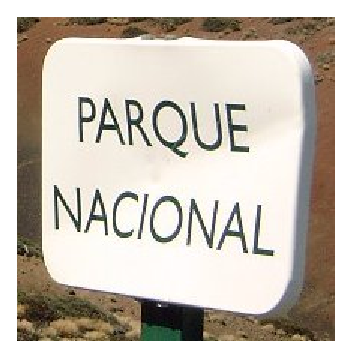
\includegraphics[scale=0.25]{parque-nacional}
    }
  }{label}
  \psline[linecolor=red](A)(B)
\end{pspicture}
\end{LTXexample}

\bigskip

\begin{LTXexample}[width=3.5cm]
\begin{pspicture}(3,3)\psgrid
  \pnode(0,0){A}
  \pnode(1.5,2){G}
  \pnode(3,1.5){B}
  \opttripole(B)(G)(A){\rput[b](0,0){text}}{label}
  \psline[linecolor=red](A)(G)(B)
\end{pspicture}
\end{LTXexample}

\medskip

\section{Fiber-Optical Components}

\subsection{Fiber}
\begin{description}
\item[\param{fiberloops}:] \paramvalue{<integer>} (\defaultparam{3})
\item[\param{fiberloopradius}:] \paramvalue{<value>} (\defaultparam{0.3})
\item[\param{fiberloopsep}:] \paramvalue{<value>} (\defaultparam{0.3})
\end{description}
\medskip

\begin{LTXexample}[width=3.5cm]
\begin{pspicture}(3,2)\psgrid
  \optfiber(0,1)(3,1){SSMF}
\end{pspicture}
\end{LTXexample}

\medskip

\subsection{Amplifier}
\begin{description}
\item[\param{optampsize}:] \paramvalue{<value>} (\defaultparam{0.8})
\end{description}

\medskip

\begin{LTXexample}[width=3.5cm]
\begin{pspicture}(3,2)\psgrid
  \optamp(0,1)(3,1){EDFA}
\end{pspicture}
\end{LTXexample}

\medskip

\subsection{Mach-Zehnder Modulator}
\begin{description}
\item[\param{optmzmsize}:] \paramvalue{<value>} (\defaultparam{0.8})
\end{description}

\medskip

\begin{LTXexample}[width=3.5cm]
\begin{pspicture}(3,2)\psgrid
  \optmzm(0,1)(3,1){MZM}
\end{pspicture}
\end{LTXexample}

\medskip

\subsection{Filter}
\begin{description}
\item[\param{filtertype}:] \paramvalue{bandpass|bandstop} (\defaultparam{bandpass})
\end{description}

\medskip

\begin{LTXexample}[width=3.5cm]
\begin{pspicture}(3,2)\psgrid
  \optfilter(0,1)(3,1){bandpass}
\end{pspicture}
\end{LTXexample}

\bigskip

\begin{LTXexample}[width=3.5cm]
\begin{pspicture}(3,2)\psgrid
  \optfilter[filtertype=bandstop](0,1)(3,1){bandstop}
\end{pspicture}
\end{LTXexample}

\medskip

\subsection{Polarization Controller}
\begin{description}
\item[\param{polcontrolsize}:] \paramvalue{<value>} (\defaultparam{0.1})
\end{description}

\medskip

\begin{LTXexample}[width=3.5cm]
\begin{pspicture}(3,2)\psgrid
  \polcontrol(0,1)(3,1){PC}
\end{pspicture}
\end{LTXexample}

\medskip

\subsection{Optical Switch}
\begin{description}
\item[\param{switchsize}:] \paramvalue{<value>} (\defaultparam{0.8})
\item[\param{switchstyle}:] \paramvalue{opened|closed} (\defaultparam{opened})
\end{description}

\medskip

\begin{LTXexample}[width=3.5cm]
\begin{pspicture}(3,2)\psgrid
  \optswitch(0,1)(3,1){Opened switch}
\end{pspicture}
\end{LTXexample}

\medskip

\begin{LTXexample}[width=3.5cm]
\begin{pspicture}(3,2)\psgrid
  \optswitch[switchstyle=closed](0,1)(3,1){Closed switch}
\end{pspicture}
\end{LTXexample}

\medskip

\subsection{Coupler}
\begin{description}
\item[\param{couplersize}:] \paramvalue{<value>} (\defaultparam{0.1})
\item[\param{couplersep}:] \paramvalue{<value>} (\defaultparam{0.1})
\item[\param{couplertype}:] \paramvalue{none|elliptic} (\defaultparam{elliptic})
\end{description}

\medskip
\subsubsection{\texorpdfstring{$2\times 2$}{2x2} Coupler}

\begin{LTXexample}[width=3.5cm]
\begin{pspicture}(3,2)\psgrid
  \optcoupler(0.5,2)(0,0.5)(3,1.5)(2.5,0){Coupler}
\end{pspicture}
\end{LTXexample}

\bigskip

\begin{LTXexample}[width=3.5cm]
\begin{pspicture}(3,2)\psgrid
  \optcoupler[align=top](0.5,2)(0,0.5)(3,1.5)(2.5,0){Coupler}
\end{pspicture}
\end{LTXexample}

\bigskip

\begin{LTXexample}[width=3.5cm]
\begin{pspicture}(3,2)\psgrid
  \optcoupler[align=bottom, couplertype=none](0.5,2)(0,0.5)(3,1.5)(2.5,0){Coupler}
\end{pspicture}
\end{LTXexample}

\medskip

\subsubsection{WDM Coupler}

\begin{LTXexample}[width=3.5cm]
\begin{pspicture}(3,2)\psgrid
  \wdmcoupler[align=bottom](0,1.5)(0,0.5)(3,0.5){WDM}
\end{pspicture}
\end{LTXexample}

\medskip

\subsubsection{WDM Splitter}
\begin{LTXexample}[width=3.5cm]
\begin{pspicture}(3,2)\psgrid
  \newpsstyle{FiberOut2}{style=Fiber, arrows=->}
  \wdmsplitter[align=top](0,1.5)(3,1.5)(3,0.5){}
\end{pspicture}
\end{LTXexample}

\medskip

\subsection{Fiber Styles}\label{sec:styles}

\begin{description}
\item[\param{usefiberstyle}:] \paramvalue{<boolean>} (\defaultparam{true})
\item[\param{Fiber}:] \paramvalue{<psstyle>} (\defaultparam{linecolor=red})
\item[\param{FiberIn}:] \paramvalue{<psstyle>} (\defaultparam{style=Fiber})
\item[\param{FiberIn1}:] \paramvalue{<psstyle>} (\defaultparam{style=FiberIn})
\item[\param{FiberIn2}:] \paramvalue{<psstyle>} (\defaultparam{style=FiberIn})
\item[\param{FiberOut}:] \paramvalue{<psstyle>} (\defaultparam{style=Fiber})
\item[\param{FiberOut1}:] \paramvalue{<psstyle>} (\defaultparam{style=FiberOut})
\item[\param{FiberOut2}:] \paramvalue{<psstyle>} (\defaultparam{style=FiberOut})
\end{description}

All these psstyles control the appearence of the fiber parts before and
after each components. The styles can be redefined with \cs{newpsstyle}
or changed with \cs{addtopsstyle}.  For optical systems it is not
possible to define a unique input and a unique output as most components
can be used bidirectionally. Therefore, I refer to the input as the part
from the first node to the component and to the output as the part from
the component to the second node.

The basic style is \parameter{Fiber} which is the parent of all other
styles. \parameter{FiberIn} inherits from \parameter{Fiber} and defines
the style of the input fiber. Analogously \parameter{FiberOut} controls
the style of the output fiber. If you want to change the input and
output fiber styles you should use \cs{addtopsstyle} as then the
inheritance from the parent style \parameter{Fiber} remains.

The other styles are used by the fiber couplers (\cs{optcoupler},
\cs{wdmcoupler} and \cs{wdmsplitter}). \parameter{FiberIn1} affects the
upper input fiber, \parameter{FiberIn2} the lower input
fiber, \parameter{FiberOut1} the upper output fiber
and \parameter{FiberOut2} the lower output fiber. If the object has only
one input (e.g. \cs{wdmsplitter}), \parameter{FiberIn} is used.

\medskip

\begin{LTXexample}[width=3.5cm]
\begin{pspicture}(3,3)\psgrid
   \addtopsstyle{FiberIn}{ArrowInside=->, arrowscale=1.2}
   \addtopsstyle{FiberOut2}{linecolor=blue}
   \optcoupler(0,2.5)(0,0.5)(3,2.5)(3,0.5){50~\%}
\end{pspicture}
\end{LTXexample}

\medskip

In addition to the psstyles there exist
corresponding \parameter{new\ldots} and \parameter{addto\ldots}
parameter keys for each of them.

\medskip

\begin{lstlisting}
\psset{addtoFiberIn={arrows=->, arrowscale=1.3}}
\end{lstlisting}

\medskip

\noindent is equivalent to 

\medskip

\begin{lstlisting}
\addtopsstyle{FiberIn}{arrows=->, arrowscale=1.3}
\end{lstlisting}

\medskip

\noindent Accordingly \parameter{newFiberIn} corresponds to \cs{newpsstyle\{FiberIn\}\{\ldots\}}.

At first glance these keys make no sense. The reason why I
introduced them was to be able to define special couplers with
\cs{newpsobject}. This is only possible if all modifications can be
expressed as parameter keys. Consider for example a WDM splitter which
only couples out a certain spectral range of the input and you want to
mark the output with an arrow:

\medskip

\begin{LTXexample}[width=3.5cm]
\begin{pspicture}(3,2)\psgrid
   \newpsobject{mywdmsplitter}{wdmsplitter}{addtoFiberOut1={arrows=->, arrowscale=1.3, linecolor=blue}, labelangle=180, align=bottom}
   \mywdmsplitter(0,0.5)(3,1.5)(3,0.5){blue band}
\end{pspicture}
\end{LTXexample}

\medskip

Or if you need a coupler with a particular input angle you can do it be extending the appropriate fiber style:

\medskip

\begin{LTXexample}[width=3.5cm]
\begin{pspicture}(3,2)\psgrid
   \newpsobject{mycoupler}{optcoupler}{addtoFiberIn2={angleA=90}, align=top}
   \mycoupler(0.5,1.5)(0.5,0.5)(2.5,1.5)(2.5,0.5){}
\end{pspicture}
\end{LTXexample}

\medskip



\section{Labels}\label{sec:labels}

\begin{description}
\item[\param{labeloffset}:] \paramvalue{<value>} (\defaultparam{1})
\item[\param{labelangle}:] \paramvalue{<value>} (\defaultparam{0})
\item[\param{labelstyle}:] \paramvalue{<macro>} (\defaultparam{\cs{small}})
\item[\param{labelalign}:] \paramvalue{<\cs{rput} ref string>} (\defaultparam{c})
\item[\param{labelref}:] \paramvalue{relative|relgrav|global} (\defaultparam{relgrav})
\end{description}

\parameter{labeloffset} specifies the offset from the center of the component, 
\parameter{labelstyle} defines the textstyle that is used to typeset the
label and \parameter{labelalign} corresponds to the refpoint of
\cs{rput}. The parameter \parameter{labelref} sets the reference
coordinate system for the \parameter{labelangle} and the orientation of
the label text. The detailed behaviour is best illustrated looking at
the following three examples.

\medskip

\begin{LTXexample}[width=5cm]
\begin{pspicture}(-2,-2)(2.5,2)
   \multido{\i=0+72}{5}{%
      \optbox[endbox,
              labelref=relative,
              labeloffset=0,
              optboxwidth=1](0,0)(1;\i){\i}
   }
\end{pspicture}
\end{LTXexample}

\bigskip

\begin{LTXexample}[width=5cm]
\begin{pspicture}(-2,-2)(2.5,2)
   \multido{\i=0+72}{5}{%
      \optbox[endbox,
              labelref=relgrav,
              optboxwidth=1](0,0)(1;\i){\i}
   }
\end{pspicture}
\end{LTXexample}

\bigskip

\begin{LTXexample}[width=5cm]
\begin{pspicture}(-2,-2)(2.5,2)
   \multido{\i=0+72}{5}{%
      \optbox[endbox,
              labelref=global,
              optboxwidth=1](0,0)(1;\i){\i}
   }
\end{pspicture}
\end{LTXexample}

\section{Defining New Components}

\subsection{Customized Versions of Existing Macros}

The easiest way to define your own components is to use the
\cs{newpsobject} macro. With this you can define a new component using
predefined objects with a set of options. These options serve only as
default values and can be overridden. The following examples defines a
new object \cs{sbn} for the special crystal used in
Sec.~\ref{sec:crystal}.

\medskip

\begin{LTXexample}[width=3.5cm]
\newpsobject{sbn}{crystal}{crystalwidth=1.5, crystalheight=0.6, voltage, lamp, labelangle=45, labeloffset=1.2, fillstyle=solid, fillcolor=yellow!90!black}
\begin{pspicture}(3,2)\psgrid 
   \sbn(0,1)(3,1){SBN:Ce}
   \psline[style=Beam](0,1)(3,1)
\end{pspicture}
\end{LTXexample}

\medskip

\begin{LTXexample}[width=3.5cm]
\newpsobject{pumpcoupler}{wdmcoupler}{align=top, labelangle=180, addtoFiberIn2={ArrowInside=->, arrowscale=2}}
\begin{pspicture}(3,2)\psgrid 
   \pumpcoupler(0,1)(0,0)(3,1){Pumpcoupler}
\end{pspicture}
\end{LTXexample}

\medskip

If you need more than one type of lenses in your setup it is very cumbersome to specify all parameters every time.

\medskip

\begin{LTXexample}[width=5.5cm]
\newpsobject{MOLensIn}{lens}{lens=0.5 0.5 0.5}
\newpsobject{MOLensOut}{lens}{lens=1.5 1.5 1.5}
\begin{pspicture}(5,2)\psgrid 
   \pnode(0,1){A}\pnode(5,1){B}
   \MOLensIn[abspos=0.5](A)(B){}
   \MOLensOut[abspos=1](A)(B){}
   \MOLensOut[abspos=4](A)(B){}
   \MOLensIn[abspos=4.5](A)(B){}
   \psline[style=Beam](A)(B)
\end{pspicture}
\end{LTXexample}
\medskip

\subsection{Defining New Objects}\label{sec:newobj}

Since version 1.2 \texttt{pst-optexp} provides some high-level macros to
allow very convenient definition of completely new components. The macro
\cs{newOptexpDipole} generates all organizing code for a new free-ray
component. All you have to do is to define a new "`drawing"' macro
\cs{mycomponent@iii} which contains all drawing code. Analogously
\cs{newOptexpDipoleNolabel} defines a new free-ray object which takes no label
(like \cs{polarization}) and \cs{newOptexpTripole} defines a new
reflective component. 

New fiber-optical components can be defined using
\cs{newOptexpFiberDipole}. This macro differs from its free-ray
analogous only in that it presets \parameter{fiber} and hence directly
connects the component with the nodes. The first node in the parameter
list gets connected with a node \parameter{tempNode@A@}, the second node
with a node \parameter{tempNode@B@}. These two internal nodes are preset
to \parameter{(0,0)} and can be overwritten within the drawing macro.

The syntax of the macros is
\begin{lstlisting}
\newOptexpDipole[fixed options]{name}{default options}
\newOptexpDipoleNolabel[fixed options]{name}{default options}
\newOptexpTripole[fixed options]{name}{default options}
\newOptexpFiberDipole[fixed options]{name}{default options}
\end{lstlisting}
The \texttt{default options} are simply a list of PSTricks parameters
which are taken as defaults for the new component. The optional argument
allows setting of parameters which cannot be overridden later.

This is illustrate a bit more in the next code snippet, which also shows
how the coordinate system is handled withing the \cs{mycomponent@iii}
macro.

\medskip

\begin{LTXexample}[width=4.5cm]
\newOptexpTripole{mygrid}{subgriddiv=5, griddots=0, subgridwidth=\pslinewidth, gridwidth=2\pslinewidth}
\makeatletter
\def\mygrid@iii{% put here all PSTricks drawing code
  \psgrid(-1,0)(1,1)
}%
\makeatother
\begin{pspicture}(4,4)\psgrid 
   \pnode(0,1){A}\pnode(2,2){G}\pnode(3,0){B}
   \mygrid[gridcolor=red,labeloffset=1.5](A)(G)(B){myGrid}
   \psline[style=Beam](A)(G)(B)
\end{pspicture}
\end{LTXexample}
\medskip

The default position of the label reference point is (0,0). If you want
to change this, you have to define a new pnode named
\texttt{tempNode@Label} in the \cs{mycomponent@iii} macro.

If you create a new component, please send it to me then I can
incorporate this in a new released version.

\newpage

\section{Examples}
\psset{unit=1.2cm}
\begin{LTXexample}[pos=t,vsep=8mm]
\begin{pspicture}(0,0.2)(12,1.8)
\pnode(0,1.2){Start}\pnode(11,1.2){CCD}
\psline[linewidth=2\pslinewidth,style=Beam](Start)(CCD)
\polarization[poltype=perp,position=0.1](Start)(CCD)
\optretplate[position=0.15](Start)(CCD){$\nicefrac{\lambda}{2}$}
\lens[lensheight=0.5,
      lensradius=0.5,
      position=0.25](Start)(CCD){$L_1$}
\lens[position=0.5](Start)(CCD){$L_2$}
\optplate[position=0.57, platelinewidth=3\pslinewidth](Start)(CCD){SLM}
\optplate[position=0.63](Start)(CCD){PF}
\polarization[position=0.66](Start)(CCD)
\lens[position=0.7](Start)(CCD){$L_3$}
\optbox[endbox,labeloffset=0](Start)(CCD){CCD}
\end{pspicture}
\end{LTXexample}

\vspace{\fill}

\begin{LTXexample}[pos=t,vsep=8mm]
\begin{pspicture}(-4,-1)(3,3)
  \psset{labeloffset=0.5}
  \pnode(-2,0){LaserOut}
  \pnode(0,0){Grid}
  \pnode(4;45){Out}
  \pnode(2.5;67.5){Mvar}
  \psline[linewidth=2\pslinewidth,
         linecolor=red!90!black](LaserOut)(Grid)(Out)\psline(Grid)(Mvar)
  \optbox[endbox, optboxwidth=2, labeloffset=0](Grid)(LaserOut){diodelaser}
  \optretplate[position=0.3, labeloffset=0.8](LaserOut)(Grid){$\nicefrac{\lambda}{4}$}
  \optgrid(LaserOut)(Grid)(Out){grid}
  \mirror[variable](Grid)(Mvar)(Grid){M$_\mathrm{var}$}
\end{pspicture}
\end{LTXexample}

\begin{LTXexample}[pos=t,vsep=3mm]
\begin{pspicture}(0,-0.4)(9,6)
  \pnode(1.5,5){Laser}\pnode(4,5){PBS}\pnode(6.5,5){PBS2}
  \pnode(6.5,5.7){piezo}\pnode(4,2){BSFwd}\pnode(6.5,2){BSBwd}
  \pnode(2,2){BS4f}\pnode(2,0.5){M4f3}\pnode(8,2){M4f1}
  \pnode(8,0.5){M4f2}\pnode(1,2){CCD}
  \psline[style=Beam,linewidth=2\pslinewidth]%
         (Laser)(PBS2)(piezo)(BSBwd)(M4f1)(M4f2)(M4f3)(BS4f)(CCD)
  \psline[style=Beam,linewidth=2\pslinewidth](PBS)(BSFwd)(BS4f)
  \psset{mirrorwidth=0.6, plateheight=0.7, outerheight=0.7, labeloffset=0.7, labelstyle=\scriptsize, lensheight=0.8, lenswidth=0.2, bssize=0.5} 
  \optbox[endbox,optboxwidth=1.5, optboxheight=0.7,labeloffset=0]%
     (PBS)(Laser){\parbox{1.5cm}{\centering Nd:YAG\\ 532\,nm}}
  \lens[lensheight=0.5, position=0.2](Laser)(PBS){MO}
  \pinhole[position=0.3,labelangle=180](Laser)(PBS){PH}
  \lens[position=0.5](Laser)(PBS){L}
  \optretplate[position=0.8](Laser)(PBS){$\nicefrac{\lambda}{2}$}
  \beamsplitter(Laser)(PBS)(BSFwd){PBS}
  \optretplate[position=0.4](PBS)(BSFwd){$\nicefrac{\lambda}{2}$}
  \polarization(PBS)(BSFwd)\polarization(PBS2)(BSBwd)
  \lens[position=0.8](PBS)(BSFwd){L}
  \optretplate(PBS)(PBS2){$\nicefrac{\lambda}{2}$}
  \beamsplitter(PBS)(PBS2)(piezo){PBS}
  \optretplate[abspos=0.5](PBS2)(piezo){$\nicefrac{\lambda}{4}$}
  \mirror[mirrortype=piezo,labelangle=90](PBS2)(piezo)(PBS2){PZ}
  \lens[position=0.8,labelangle=180](PBS2)(BSBwd){L}
  \beamsplitter(PBS)(BSFwd)(BSBwd){BS}
  \beamsplitter[labelangle=-90](PBS2)(BSBwd)(BSFwd){BS}
  \crystal[crystalwidth=1, crystalheight=0.5, voltage, lamp, fillstyle=solid, fillcolor=yellow!90!black, labeloffset=0.8](BSFwd)(BSBwd){SBN:Ce}
  \mirror(BSBwd)(M4f1)(M4f2){M}\mirror(M4f1)(M4f2)(M4f3){M}
  \lens[labelangle=180](M4f2)(M4f3){L}\mirror(M4f2)(M4f3)(BS4f){M}
  \beamsplitter(M4f3)(BS4f)(CCD){BS}\optbox[endbox,labeloffset=0](BS4f)(CCD){CCD}
  \lens[abspos=0.7](BS4f)(BSFwd){L}\lens[abspos=0.7](BSBwd)(M4f1){L}
  \psline[style=Beam, linewidth=2\pslinewidth](BSFwd)(BSBwd)
\end{pspicture}
\end{LTXexample}

The following schematic configuration of a recirculating loop was
adapted from the publication N. Kikuchi, S. Sasaki and K. Sekine, "`10
Gbit/s dispersion-compensated transmission over 2245~km conventional
fibres in a recirculating loop"', Electron. Lett. 31 (\textbf{5}), 375
(1995).

\begin{LTXexample}[pos=t]
\psset{unit=1cm}
\begin{pspicture}(0.5,4)(13.2,10.5)
  \laser[labeloffset=0](2.1,10)(2,10){LD}
  \optmzm(2.1,10)(3.5,10){MZM}
  \optamp(3.5,10)(4.5,10){EDFA}
  \optfilter(4.5,10)(5.5,10){BPF}
  \optswitch(5.5,10)(6.5,10){SW}
  \polcontrol(6.5,10)(7.5,10){}
  \optcoupler[couplertype=none,couplersep=0.2](7.5,10)(7.5,8)(9,10)(9,8){}
  \optamp(9,10)(10.5,10){EDFA}
  \optfilter(10.5,10)(12,10){BPF}
  \optbox[endbox, labeloffset=0, conn=f-f](12,10)(12.1,10){RX}
  % loop
  \optamp(9,8)(11,8){EDFA}
  \psline[linearc=1,style=Fiber](11,8)(12,8)(12,4.5)(11,4.5)
  \optfiber[labelalign=b, labeloffset=-1, position=0.8](9,4.5)(11,4.5){\begin{tabular}{c}conventional\\fibre 89.8~km\end{tabular}}
  \optamp(9,4.5)(8,4.5){EDFA}
  \optfilter(8,4.5)(6.5,4.5){BPF}
  \optfiber[fiberloops=1, labeloffset=-1, labelalign=b](4,4.5)(6.5,4.5){DCF 16.2~km}
  \optamp(4,4.5)(2.5,4.5){EDFA}
  \psline[style=Fiber,linearc=1](2.5,4.5)(1.5,4.5)(1.5,8)(2.5,8)
  \optfilter(2.5,8)(4.5,8){BPF}
  \optswitch(4.5,8)(6,8){SW}
  \polcontrol(6,8)(7.5,8){}
\end{pspicture}
\end{LTXexample}

\newpage

\section{Complete List of Parameters}
\begin{longtable}{BTT}
\toprule \multicolumn{1}{l}{parameter} & \multicolumn{1}{l}{values} & \multicolumn{1}{l}{default}\\\midrule\endhead
\bottomrule\endfoot
\input alphabetical-option-list
\end{longtable}
\newpage
\section{Todo}

The next thing I will add are components with multiple internal
reflections, as right-angle, penta and dove prisms. The code is almost
ready, I just need to think a bit more about the best way to provide
access to the nodes that are newly defined within the components.

Drawing of extended beams with focusing and so on could be integrated to
some extent in future versions. But as the topic is rather difficult if
you want to do it properly (components should be placed above the beam,
but the new nodes are available only when the component is drawn) it
could take very long until this feature will be implemented.

\section{Acknowledgements}

I thank all the people of the PSTricks mailinglist for the continuous help, especially Herbert Vo�.

\section{History}

For the package history see file Changes that is distributed with the package.
\end{document}
